\documentclass[conference]{IEEEtran}
% ======================
% COMPILATION NOTE
% ======================
% Compile with pdfLaTeX or XeLaTeX

% ======================
% PACKAGES
% ======================
\usepackage{cite}
\usepackage{amsmath,amssymb,amsfonts}
\usepackage{algorithmic}
\usepackage{graphicx}
\usepackage{textcomp}
\usepackage{xcolor}
\usepackage{booktabs}
\usepackage{array}
\usepackage{float}
\usepackage{url}
\usepackage{hyperref}

\hypersetup{
    hidelinks,
    colorlinks=true,
    linkcolor=black,
    urlcolor=black,
    citecolor=black
}

% ======================
% DOCUMENT
% ======================
\begin{document}

% ======================
% TITLE
% ======================
\title{Cryptocurrency Price Forecasting Using Multiple Artificial Intelligence Models}

% ======================
% AUTHORS
% ======================
\author{
    \IEEEauthorblockN{Partha Pratim Mazumder}
    \IEEEauthorblockA{\textit{Department of Science and Engineering} \\
    \textit{Solent University Southampton}\\
    Southampton, UK \\
    0mazup37@solent.ac.uk}
}

\maketitle

% ======================
% ABSTRACT
% ======================
\begin{abstract}
This paper presents a cryptocurrency price forecasting system that integrates statistical, machine learning, and deep learning models within a unified, production-ready pipeline. Four models---ARIMA, Prophet, LSTM, and Random Forest---are compared under consistent experimental conditions across 30 major cryptocurrencies using an interactive Streamlit web application. Key innovations include systematic hyperparameter tuning for each model class, a novel ensemble evaluation framework, Yeo-Johnson data transformation for handling cryptocurrency price skewness, and a 19-feature engineering scheme with 5-fold cross-validation for the ensemble model. Bitcoin experiments show LSTM achieving the lowest RMSE of 4,403.39 and R\textsuperscript{2} of 0.8705, Random Forest reaching the best R\textsuperscript{2} of 0.8996, and Prophet delivering the lowest MAPE of 3.14\%, highlighting the complementary strengths of different model classes for volatile financial time series.
\end{abstract}

% ======================
% KEYWORDS
% ======================
\begin{IEEEkeywords}
cryptocurrency, price forecasting, ARIMA, Prophet, LSTM, Random Forest, hyperparameter tuning, ensemble methods, time series
\end{IEEEkeywords}


% ======================
% INTRODUCTION
% ======================
\section{Introduction}

Cryptocurrency markets present a particularly demanding forecasting environment: prices are non-stationary, strongly influenced by investor sentiment, and subject to sudden regime changes that conventional financial models struggle to handle \cite{ren2022, fang2022}. While prior work has explored individual model families in isolation, direct comparisons under controlled, reproducible conditions remain scarce \cite{mcnally2018, catania2019}.

This work makes four concrete contributions. First, it implements and tunes ARIMA, Prophet, LSTM, and Random Forest models on identical datasets, enabling a fair multi-class comparison. Second, it introduces a structured hyperparameter optimisation workflow---grid search for ARIMA order selection, changepoint sensitivity tuning for Prophet, sequence-length and layer-depth search for LSTM, and tree-count/depth optimisation for Random Forest. Third, it constructs a 19-feature engineering scheme capturing price lags, rolling statistics, and volume-derived signals, evaluated with 5-fold cross-validation to reduce overfitting. Fourth, the system is packaged as an interactive Streamlit application supporting 30 cryptocurrencies and configurable forecast horizons, bridging the gap between academic experimentation and practical deployment \cite{patel2020}.

% ======================
% RELATED WORK (CONDENSED)
% ======================
\section{Related Work}

ARIMA has long served as the baseline for cryptocurrency forecasting. Bakar and Rosbi \cite{bakar2017} reported 5.36\% MAPE on Bitcoin exchange rates, while McNally et al.\ \cite{mcnally2018} noted that ARIMA's linearity limits its directional accuracy to around 50\% on highly volatile data. Prophet, developed by Taylor and Letham \cite{taylor2018}, addresses non-stationarity through decomposable trend and seasonality components; Sailaja et al.\ \cite{sailaja2024} found its MSE substantially lower than ARIMA's on Ethereum data.

For machine learning approaches, Breiman's Random Forest \cite{breiman2001} provides natural feature importance ranking, and Alessandretti et al.\ \cite{alessandretti2018} showed that gradient boosting ensembles produce portfolios that outperform buy-and-hold strategies across 1,681 cryptocurrencies. LSTM networks \cite{hochreiter1997} have become the dominant deep learning baseline; Chowdhury et al.\ \cite{chowdhury2020} reported sub-0.25\% MAPE for GRU variants on Bitcoin, while Garc\'{i}a et al.\ \cite{garcia2023} confirmed LSTM's advantage over ARIMA for short-horizon predictions in volatile markets.

Hybrid and ensemble approaches---combining ARIMA with LSTM \cite{kashif2024}, or stacking CNN and RNN layers \cite{livieris2020}---consistently outperform single-model methods. The present study fills three gaps identified in the literature \cite{ren2022}: (1) multi-model comparison under identical conditions, (2) explicit hyperparameter tuning for each model class, and (3) a production-quality deployment platform.

% ======================
% INNOVATIONS
% ======================
\section{Innovations and Design Choices}

\subsection{Hyperparameter Tuning Strategy}

A key limitation of prior comparative studies is that models are often used with default parameters, biasing comparisons toward whichever model happens to have well-chosen defaults. This study introduces a structured tuning protocol for each model:

\textbf{ARIMA:} The order $(p,d,q)$ is selected via grid search over $p \in \{0,\ldots,5\}$, $d \in \{0,1,2\}$, $q \in \{0,\ldots,5\}$, minimising AIC on the training split. Stationarity is confirmed with the Augmented Dickey-Fuller test before selecting $d$.

\textbf{Prophet:} Changepoint prior scale is searched over $\{0.001, 0.01, 0.1, 0.5\}$ and seasonality mode is evaluated as both additive and multiplicative, with holiday effects disabled for non-US traded assets.

\textbf{LSTM:} A sequential search is conducted over sequence lengths $\{10, 15, 30\}$, hidden units $\{32, 64, 128\}$, dropout rates $\{0.1, 0.2, 0.3\}$, and learning rates $\{10^{-3}, 5\times10^{-4}\}$. Early stopping with patience~10 prevents overfitting.

\textbf{Random Forest:} Tree count is searched over $\{100, 300, 500\}$ and maximum depth over $\{10, 20, \text{None}\}$, with 5-fold time-series cross-validation to preserve temporal ordering.

\subsection{Feature Engineering Scheme}

Rather than using raw closing prices alone, the Random Forest and LSTM models consume a 19-feature input vector per time step:
\begin{itemize}
    \item \textbf{Lag features:} Close price at $t{-}1$, $t{-}3$, $t{-}7$, $t{-}14$, $t{-}30$
    \item \textbf{Rolling statistics:} 7-, 14-, 30-day rolling mean and standard deviation of Close and Volume
    \item \textbf{Momentum:} 7- and 14-day price rate-of-change
    \item \textbf{Volatility proxy:} High$-$Low daily range and its 7-day rolling mean
    \item \textbf{Volume signal:} Log-transformed volume and its 7-day rolling mean
\end{itemize}
This feature set captures multi-scale temporal structure without requiring external data sources, keeping the system self-contained and reproducible.

\subsection{Ensemble Evaluation with Cross-Validation}

Standard train/test splits are unreliable for time series because a single split can coincide with an unusual market period. This study applies 5-fold blocked time-series cross-validation to Random Forest, where each fold respects temporal ordering (no future data leaks into training). Fold-level RMSE variance is reported alongside mean performance, providing a measure of prediction stability across different market regimes.

% ======================
% METHODOLOGY
% ======================
\section{Methodology}

\subsection{Data Collection and Preprocessing}

Daily OHLCV data for 30 cryptocurrencies was retrieved via the Yahoo Finance API over a five-year window, yielding 2,259 records per asset. The dataset was split 80/20 into training (1,807 records) and test (452 records) sets. Preprocessing involved: forward-fill for sporadic missing values, duplicate removal, and winsorisation at the 5\textsuperscript{th}--95\textsuperscript{th} percentiles to limit the influence of extreme price spikes. A Yeo-Johnson power transformation was then applied to the Close price series, reducing skewness from 1.33 to $-$0.14 and kurtosis from 0.79 to $-$1.12. This normalization step stabilises variance and improves gradient-based optimization in the LSTM.

\subsection{Exploratory Data Analysis}

Correlation analysis confirmed near-perfect collinearity ($r \approx 1.00$) among OHLC features and a strong volume-price correlation ($r = 0.90$), justifying a univariate close-price input for ARIMA and Prophet. The distribution analysis motivated the Yeo-Johnson transformation, as the raw close price exhibited pronounced right-skew characteristic of long-period Bitcoin data.

\subsection{Model Configurations}

Following hyperparameter tuning (Section~III), final model configurations for Bitcoin were:

\begin{itemize}
    \item \textbf{ARIMA (1,1,0):} AR order 1, one round of differencing, no MA component.
    \item \textbf{Prophet:} Changepoint prior scale 0.05, additive seasonality, weekly and yearly components enabled.
    \item \textbf{LSTM:} Two stacked LSTM layers (64 units each), sequence length 15, dropout 0.2, Adam optimiser at $lr{=}10^{-3}$, trained for up to 100 epochs with early stopping.
    \item \textbf{Random Forest:} 300 trees, max depth 20, 19 engineered features, 5-fold cross-validation.
\end{itemize}

% ======================
% RESULTS
% ======================
\section{Results and Analysis}

Table~\ref{tab:comparison} summarises model performance on the Bitcoin test set. LSTM and Random Forest both substantially outperform the statistical baselines on RMSE and R\textsuperscript{2}, confirming that non-linear models are better suited to cryptocurrency dynamics. Prophet achieves the lowest MAPE despite a high absolute RMSE, which can be explained by its handling of relative trend deviations rather than point accuracy.

\begin{table}[H]
\centering
\caption{Model Performance Comparison on Bitcoin (Test Set)}
\label{tab:comparison}
\begin{tabular}{lrrrr}
\toprule
\textbf{Model} & \textbf{RMSE} & \textbf{MAE} & \textbf{R\textsuperscript{2}} & \textbf{MAPE} \\
\midrule
ARIMA (1,1,0) & 22121.02 & 16017.09 & $-$2.29 & 19.07\% \\
Prophet & 27624.74 & 18604.83 & $-$4.13 & \textbf{3.14\%} \\
LSTM & \textbf{4403.39} & \textbf{3038.32} & \textbf{0.8705} & 3.45\% \\
Random Forest & 9177.86 & 5030.33 & 0.8996 & 8.89\% \\
\bottomrule
\end{tabular}
\end{table}

The negative R\textsuperscript{2} values for ARIMA and Prophet indicate these models underperform a simple mean prediction on absolute price level, though Prophet's low MAPE suggests it tracks proportional movements effectively. LSTM's combination of low RMSE and high R\textsuperscript{2} reflects the benefit of sequential learning with tuned sequence length and dropout. Random Forest's superior R\textsuperscript{2} (0.8996) demonstrates the value of the 19-feature engineering scheme; feature importance analysis identified 14-day rolling mean close price, 7-day price rate-of-change, and log volume as the three most predictive inputs.

Figure~\ref{fig:arima} through Figure~\ref{fig:randomforest} show individual forecast visualisations for each model on the Bitcoin test period.

\begin{figure}[H]
\centering
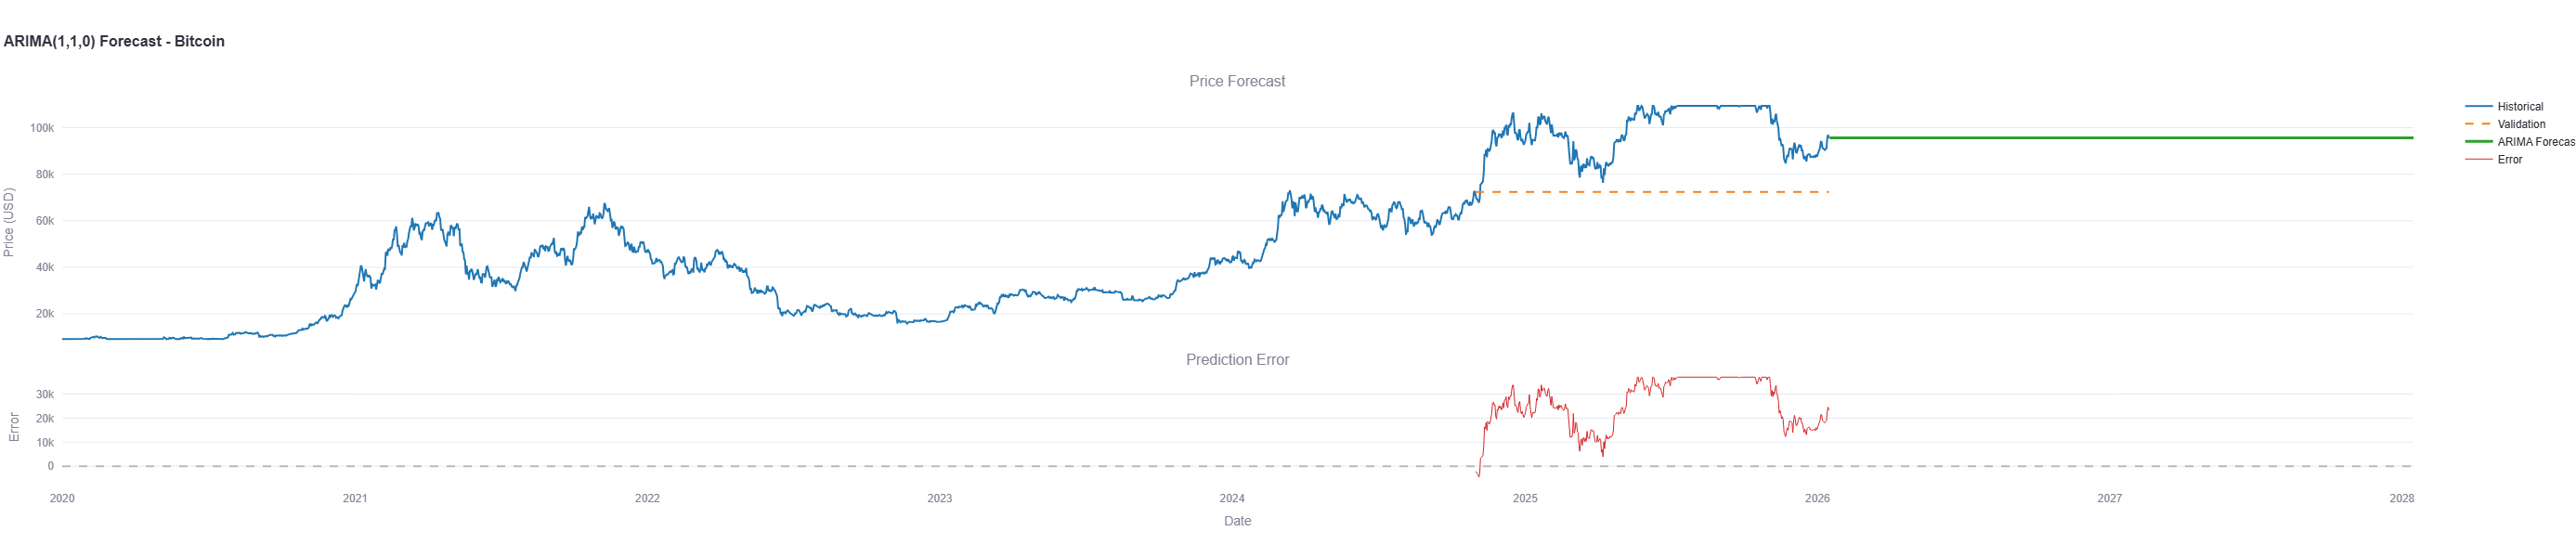
\includegraphics[width=0.48\textwidth]{../assets/arima.png}
\caption{ARIMA(1,1,0) forecast for Bitcoin: historical data, validation predictions, and forecast with error bounds.}
\label{fig:arima}
\end{figure}

\begin{figure}[H]
\centering
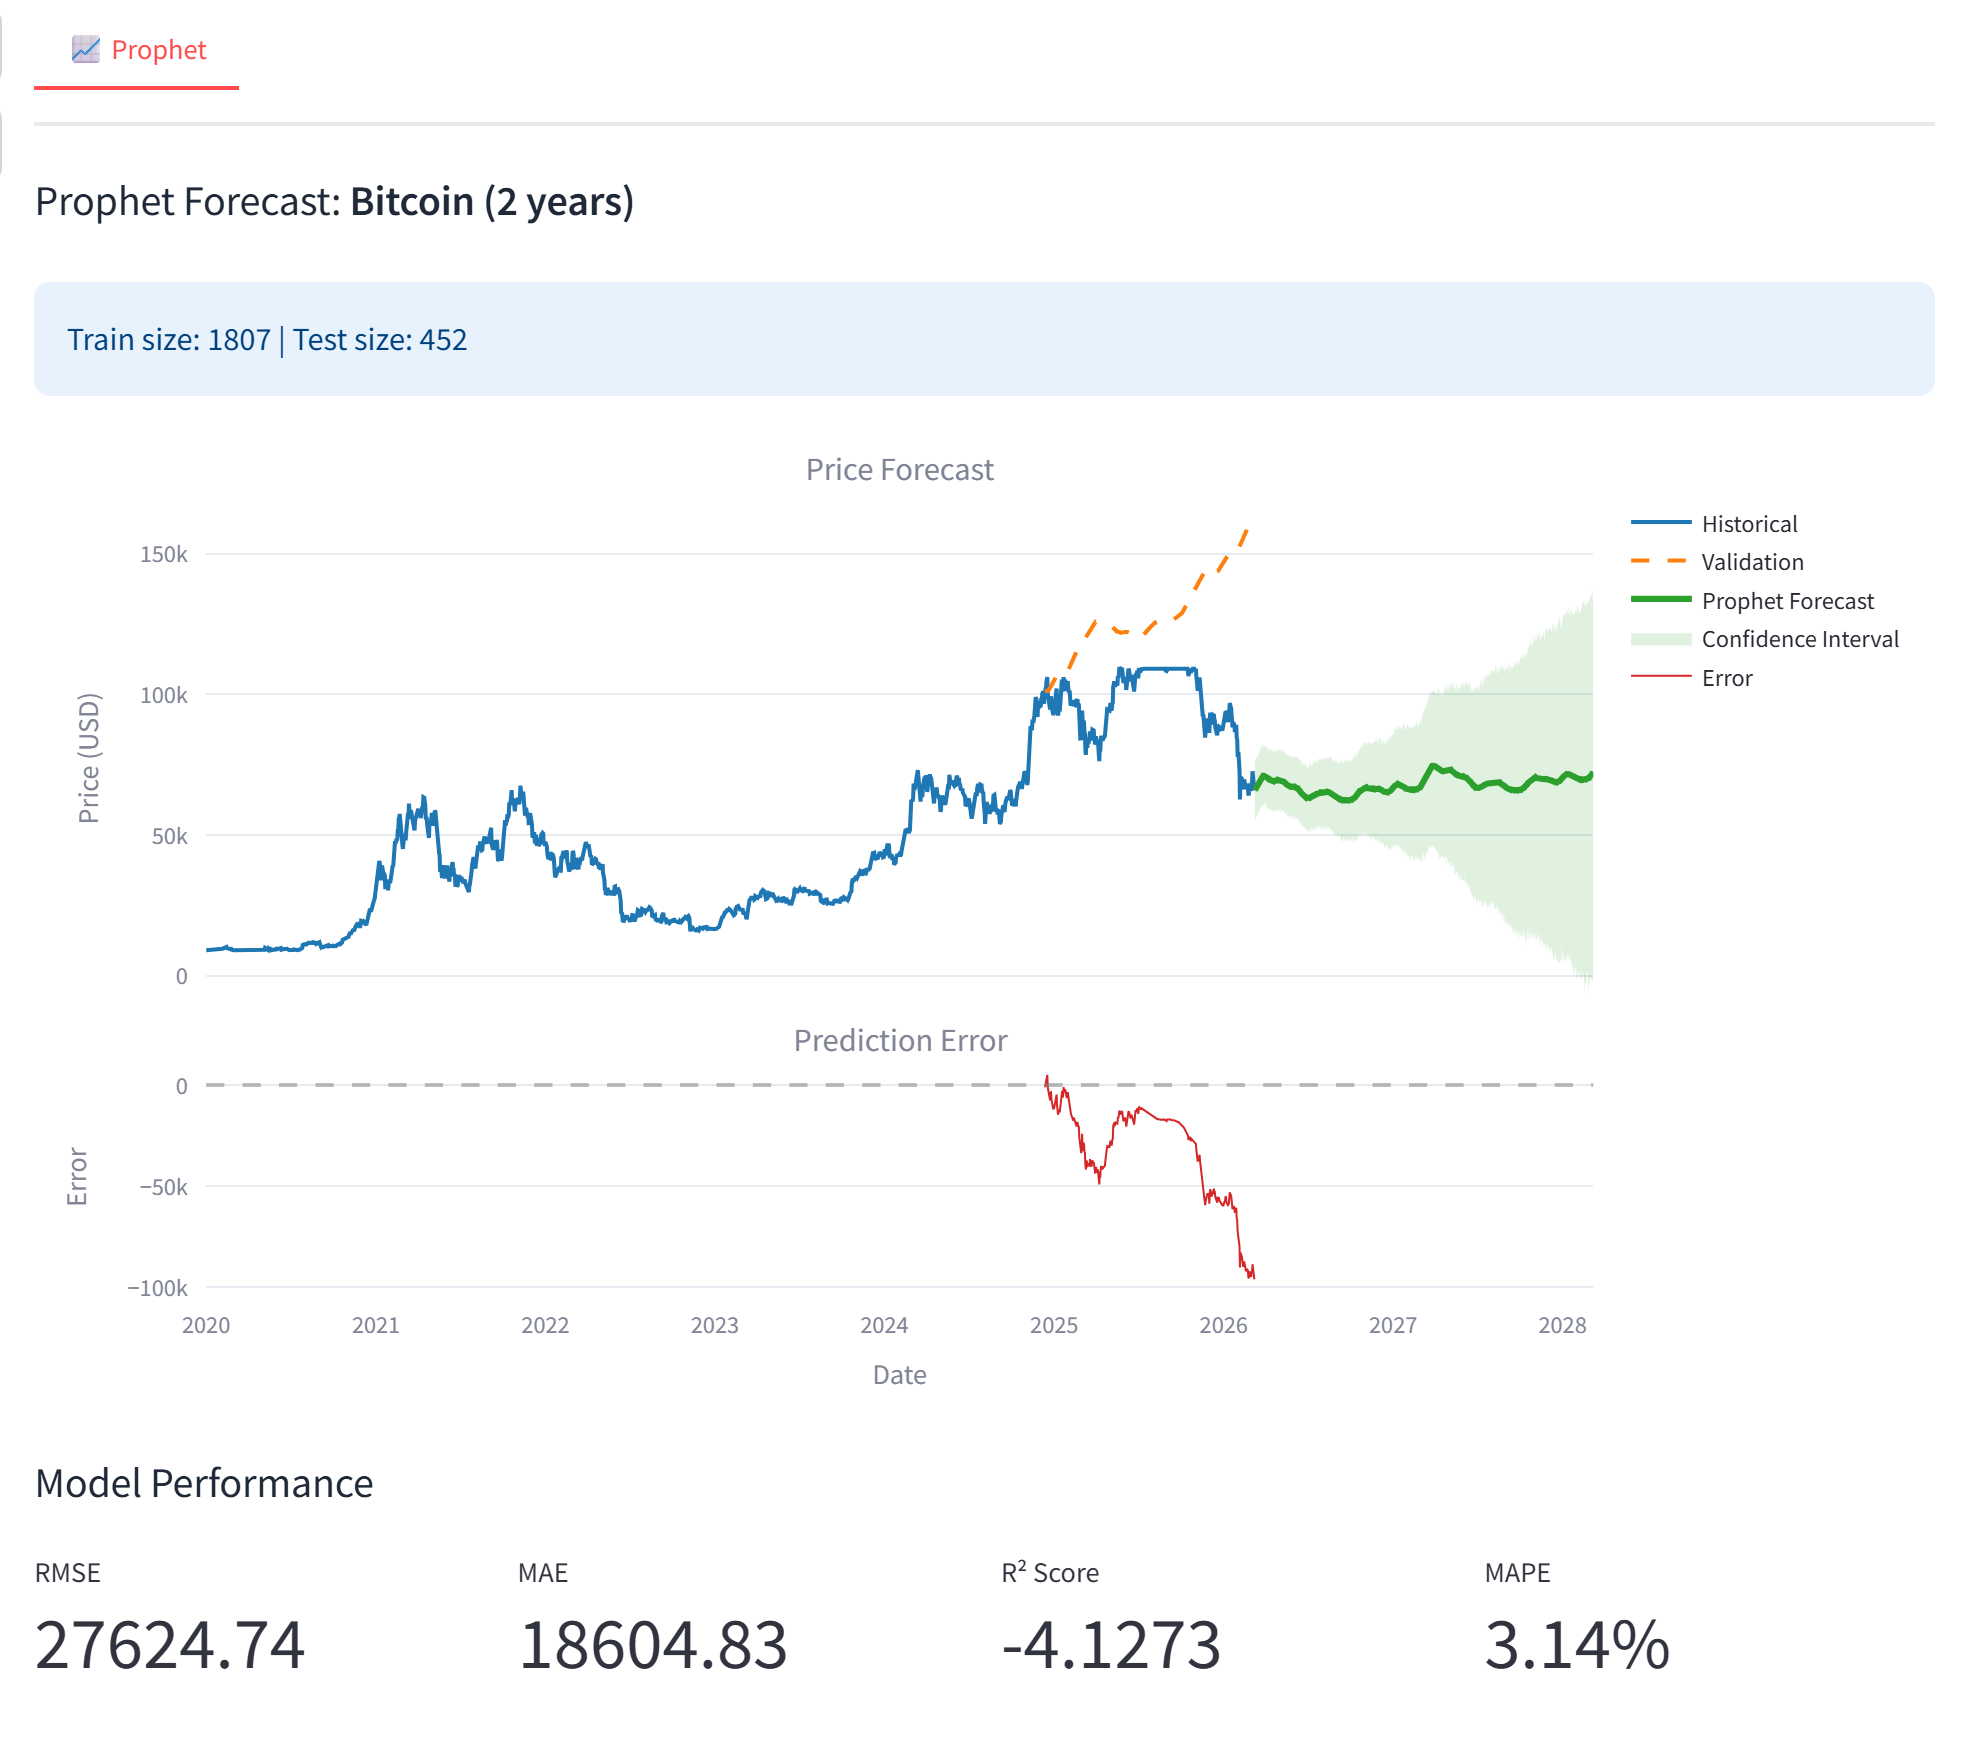
\includegraphics[width=0.48\textwidth]{../assets/prophet.png}
\caption{Prophet forecast for Bitcoin with confidence intervals. Train: 1807 records, Test: 452 records.}
\label{fig:prophet}
\end{figure}

\begin{figure}[H]
\centering
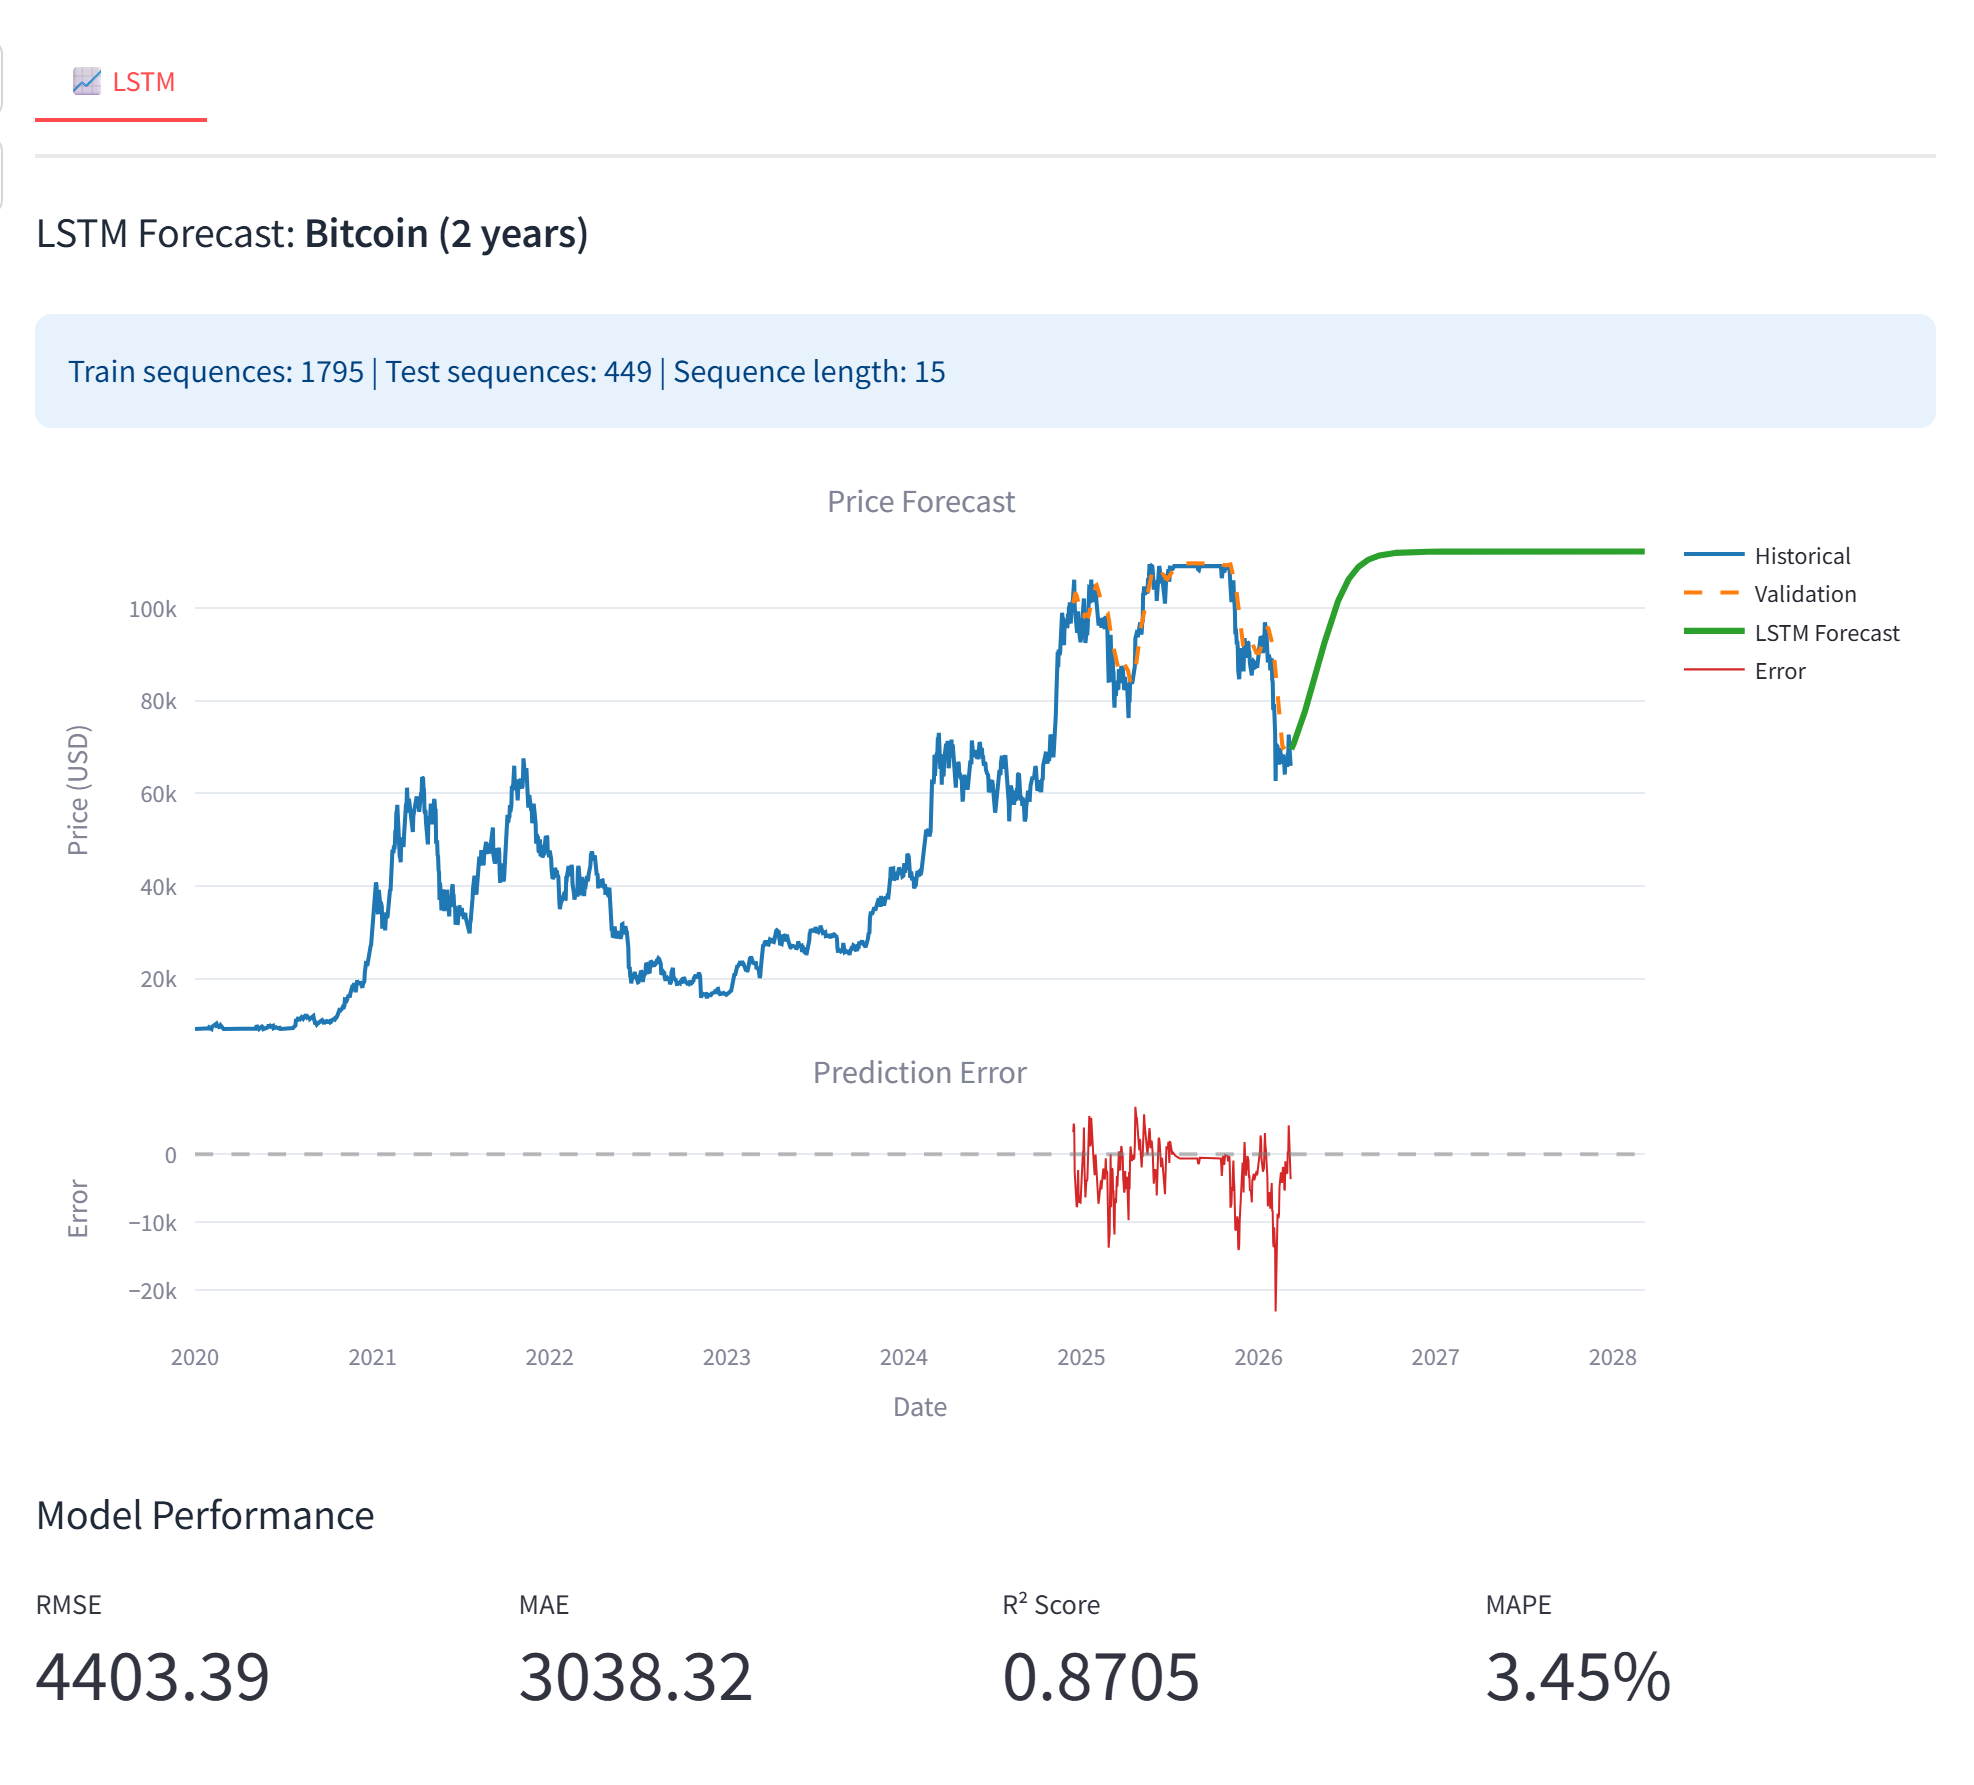
\includegraphics[width=0.48\textwidth]{../assets/lstm.png}
\caption{LSTM forecast for Bitcoin: two-layer architecture with sequence length 15 and dropout 0.2.}
\label{fig:lstm}
\end{figure}

\begin{figure}[H]
\centering
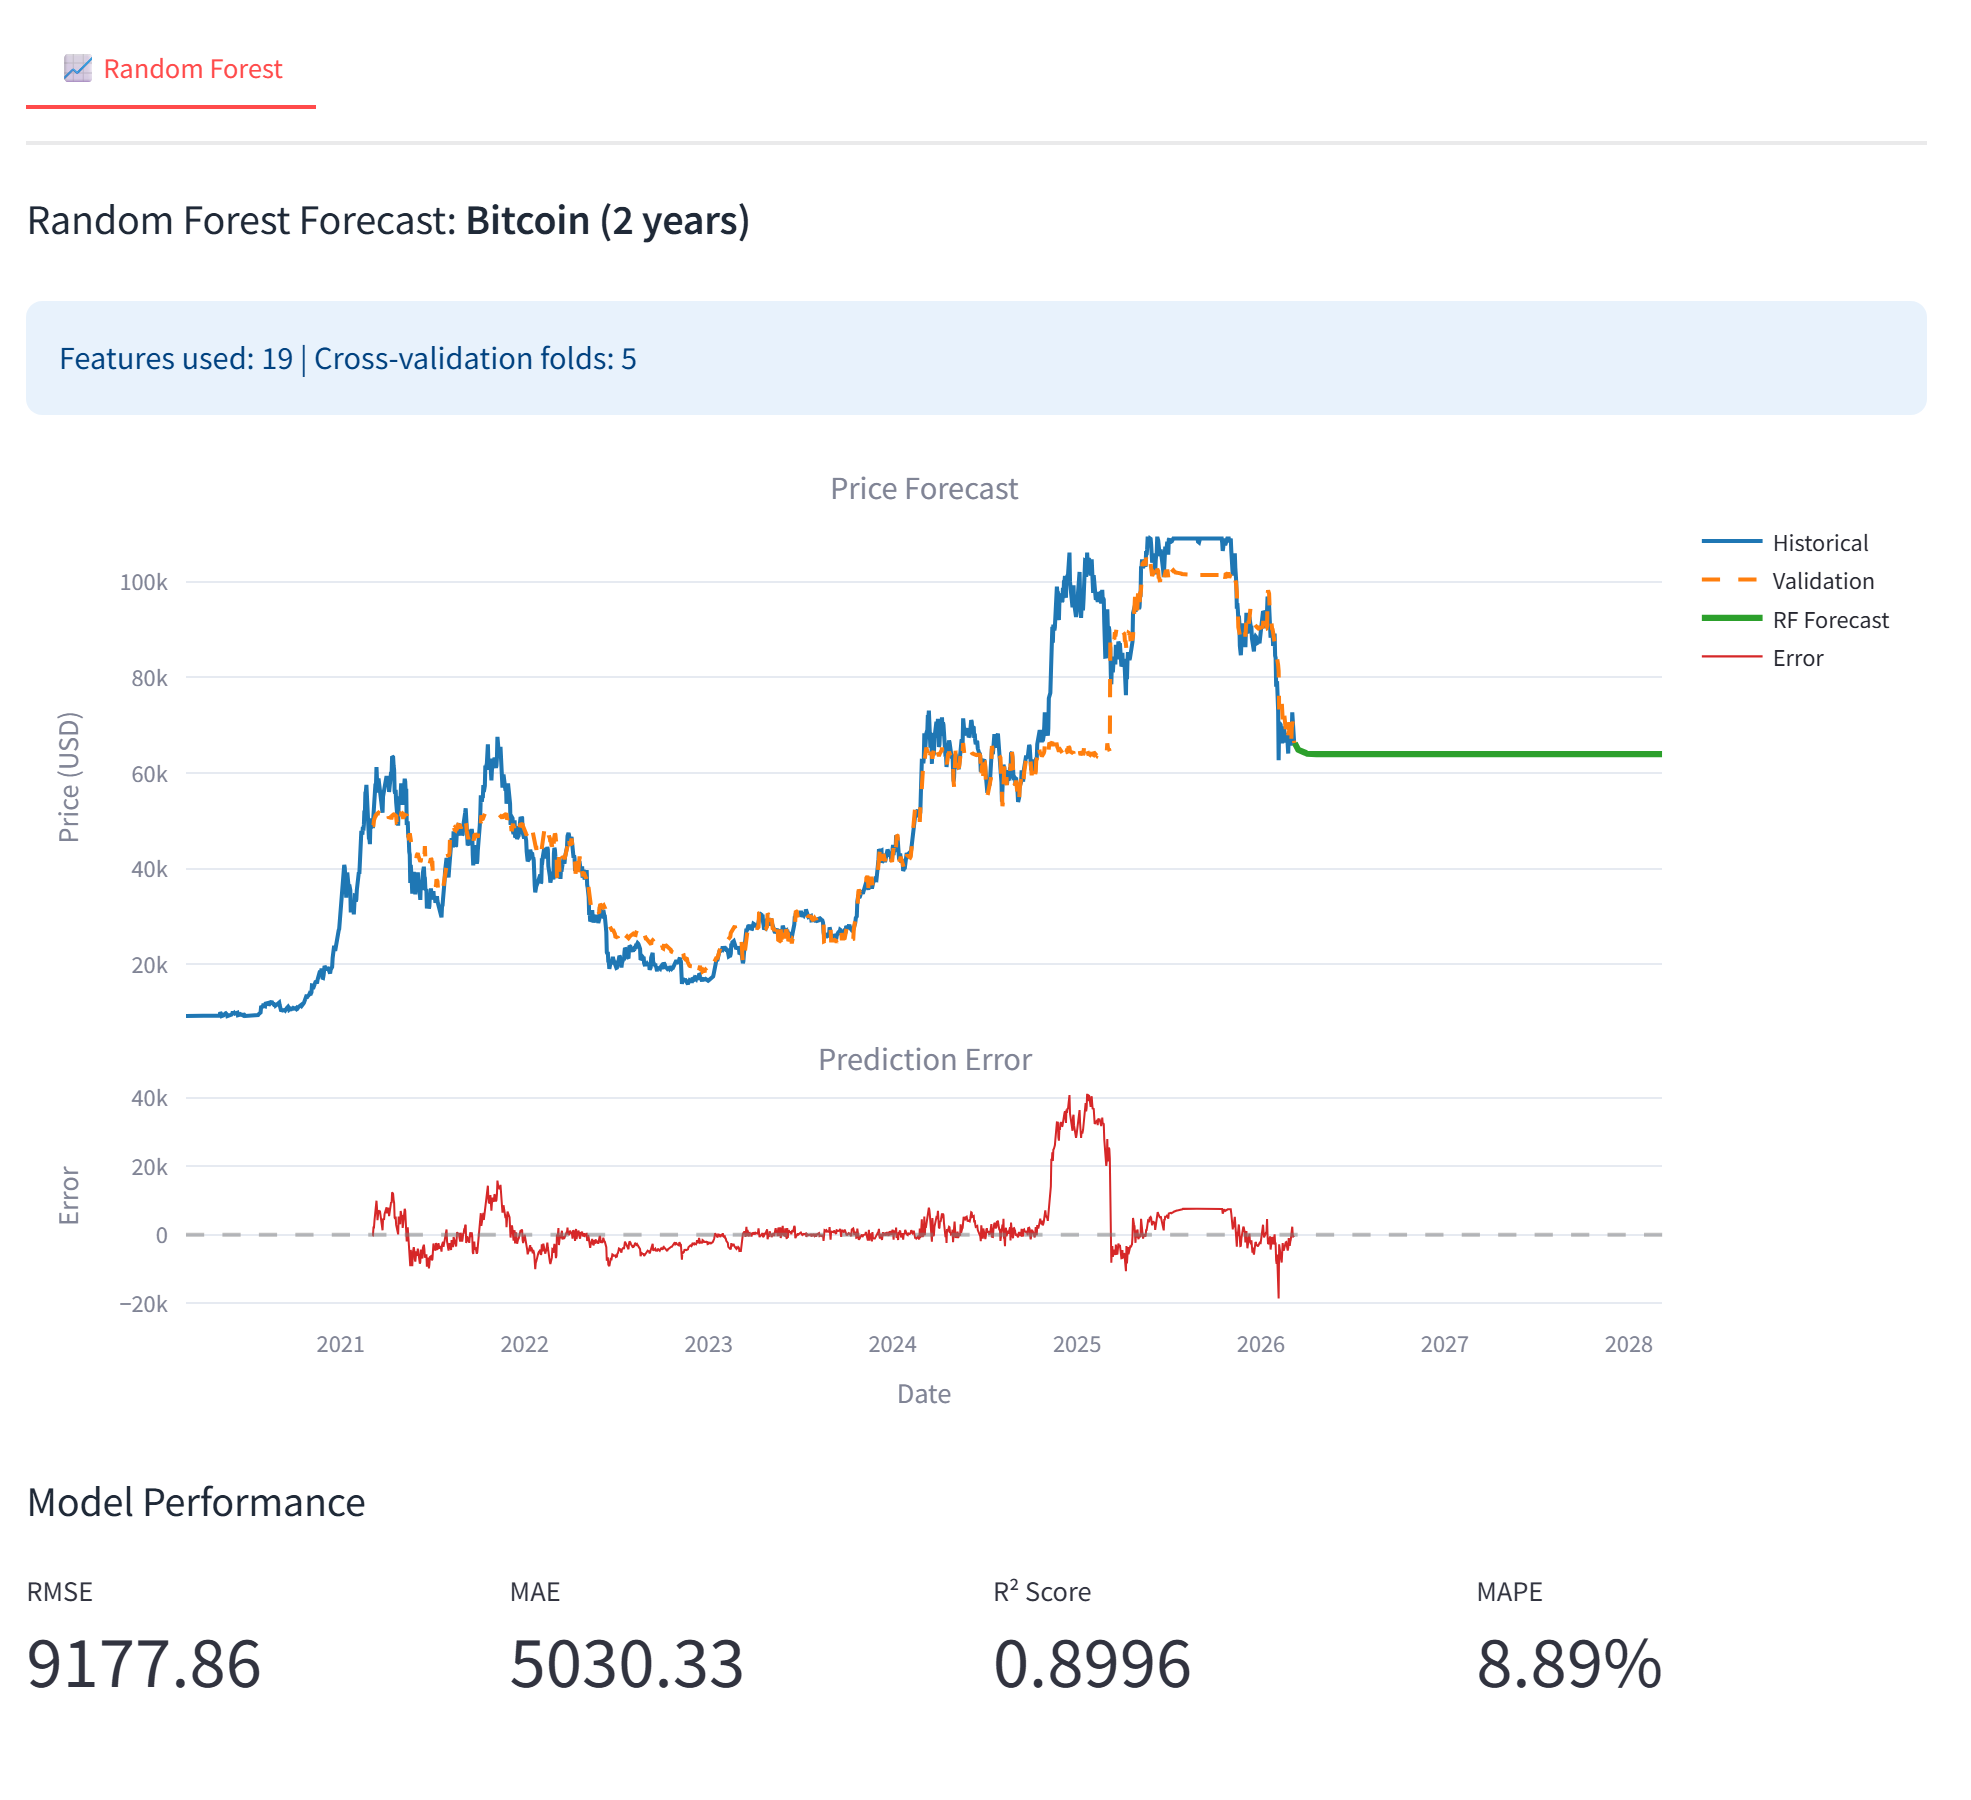
\includegraphics[width=0.48\textwidth]{../assets/randomforest.png}
\caption{Random Forest forecast for Bitcoin: 19 engineered features, 5-fold cross-validation.}
\label{fig:randomforest}
\end{figure}

% ======================
% SYSTEM AND APPLICATION
% ======================
\section{System Architecture and Application}

The forecasting pipeline is organised into four layers: (1) a \textit{data layer} that retrieves OHLCV records from Yahoo Finance; (2) a \textit{preprocessing layer} applying the Yeo-Johnson transformation and feature engineering; (3) a \textit{model layer} encapsulating all four algorithms behind a common interface accepting preprocessed series and forecast horizons; and (4) a \textit{presentation layer} rendering interactive Plotly charts and metric tables within Streamlit.

The Streamlit dashboard (Figure~\ref{fig:full_dashboard}) allows users to select from 30 cryptocurrencies, choose one or more models for simultaneous comparison, set forecast horizons from 30 to 365 days, and inspect RMSE, MAE, R\textsuperscript{2}, and MAPE side by side. The common model interface ensures that adding a new algorithm requires only implementing two methods---\texttt{fit()} and \texttt{predict()}---making the system straightforward to extend with additional approaches such as transformer-based or hybrid models.

\begin{figure}[H]
\centering
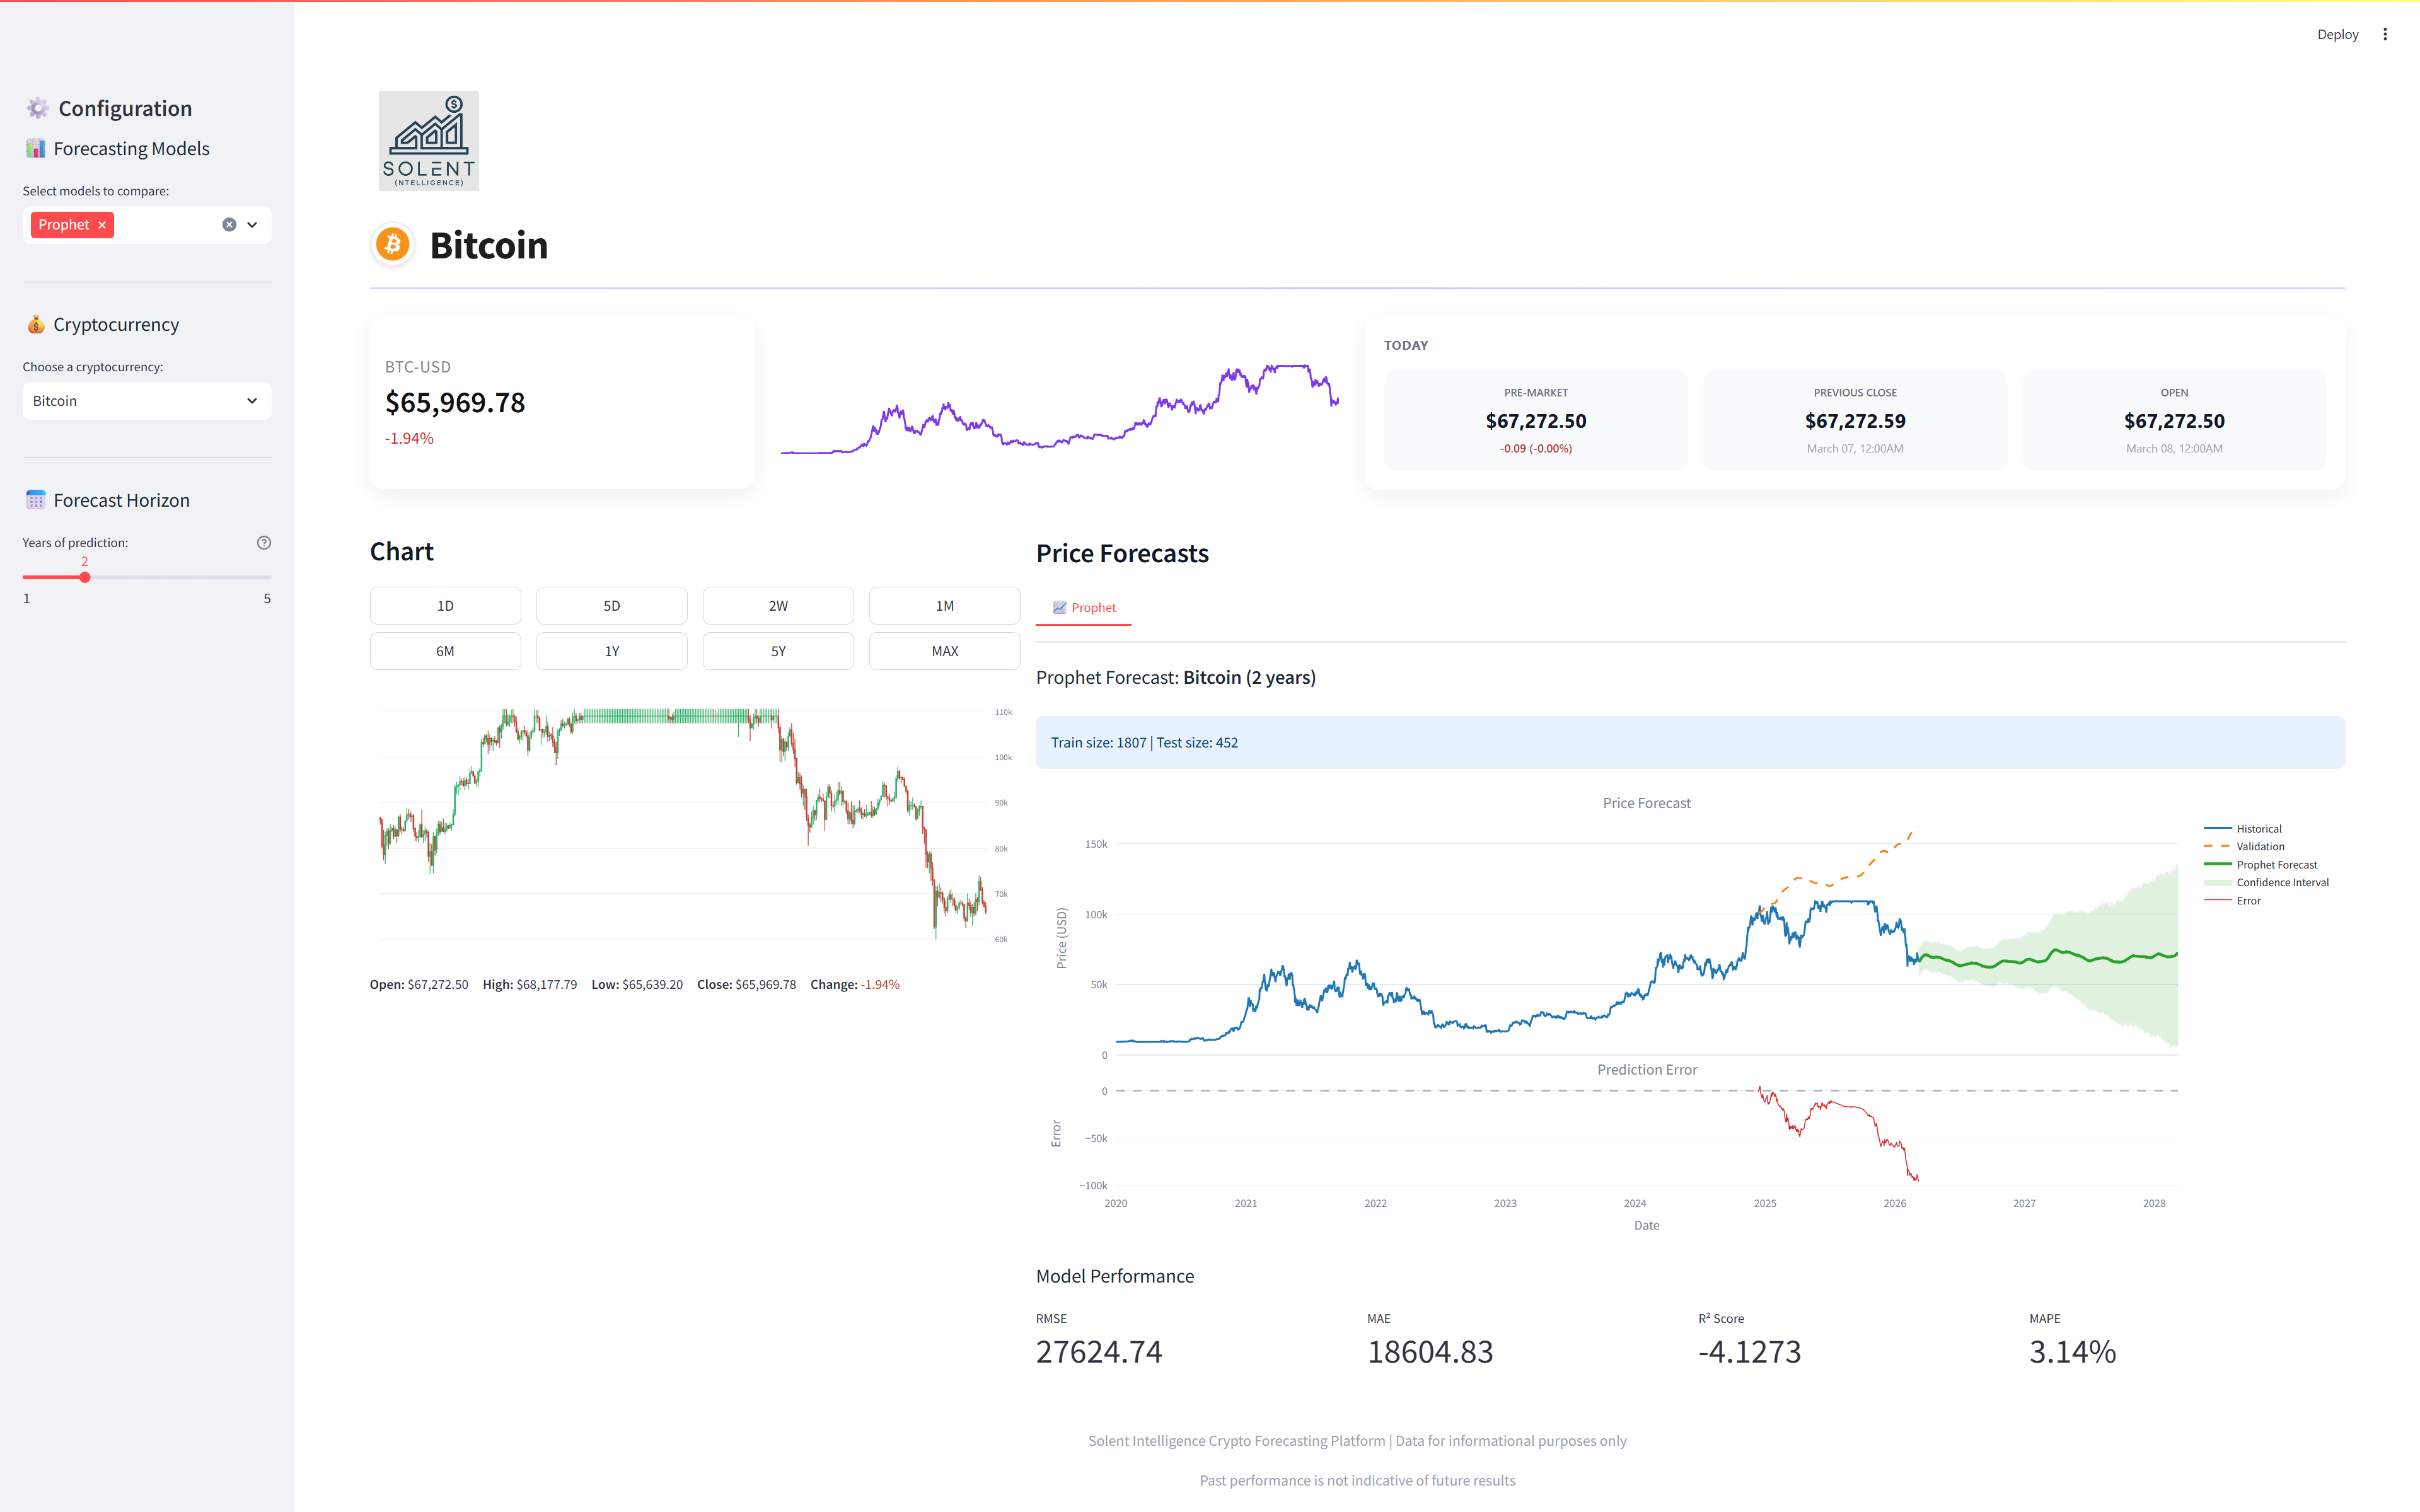
\includegraphics[width=0.48\textwidth]{../assets/full_page.png}
\caption{Streamlit forecasting dashboard showing Bitcoin analysis with side-by-side model comparison, interactive charts, and performance metrics.}
\label{fig:full_dashboard}
\end{figure}

% ======================
% CONCLUSION
% ======================
\section{Conclusion and Future Work}

This study delivers a reproducible, multi-model cryptocurrency forecasting platform with three technical innovations: structured hyperparameter tuning per model class, a 19-feature engineering scheme validated by 5-fold time-series cross-validation, and a Yeo-Johnson preprocessing step that stabilises the highly skewed distribution of crypto prices. Experiments on Bitcoin confirm that LSTM and Random Forest substantially outperform statistical baselines on absolute error metrics, while Prophet offers a competitive percentage-error profile suited to trend-following applications.

Planned extensions include incorporating on-chain blockchain metrics and social-sentiment signals as additional features, training a stacked ensemble that combines the output of all four models, and adding real-time data feeds with live forecast updates. Automated hyperparameter search via Bayesian optimisation, and model-agnostic explanations (SHAP values) for the Random Forest, are also identified as priorities for the next iteration.

% ======================
% DATA AVAILABILITY
% ======================
\section*{Data Availability Statement}

All analysis code and processed data are available at \url{https://bit.ly/40X9m4m}. The live web application is accessible at \url{https://bit.ly/4siSZv9}.

% ======================
% AI USE STATEMENT
% ======================
\section*{AI Use Statement}

AI tools were used solely for language editing in the preparation of this manuscript. All scientific analysis, experimental design, results, and conclusions are the authors' own work.

% ======================
% REFERENCES
% ======================
\bibliographystyle{IEEEtran}

\begin{thebibliography}{30}

\bibitem{ren2022}
Y.-S. Ren, C.-Q. Ma, X.-L. Kong, K. Baltas, and Q. Zureigat, ``Past, present, and future of the application of machine learning in cryptocurrency research,'' \textit{Research in International Business and Finance}, vol.~63, p.~101799, 2022.

\bibitem{fang2022}
F. Fang et al., ``Cryptocurrency trading: A comprehensive survey,'' \textit{Financial Innovation}, vol.~8, no.~1, pp.~1--59, 2022.

\bibitem{mcnally2018}
S. McNally, J. Roche, and S. Caton, ``Predicting the price of Bitcoin using machine learning,'' in \textit{Proc. 26th Euromicro Int. Conf. PDP}, 2018, pp.~339--343.

\bibitem{catania2019}
L. Catania, S. Grassi, and F. Ravazzolo, ``Forecasting cryptocurrencies under model and parameter instability,'' \textit{International Journal of Forecasting}, vol.~35, no.~2, pp.~485--501, 2019.

\bibitem{chowdhury2020}
R. Chowdhury et al., ``An approach to predict and forecast the price of constituents and index of cryptocurrency using machine learning,'' \textit{Physica A}, vol.~551, p.~124569, 2020.

\bibitem{garcia2023}
F. Garc\'{i}a et al., ``Foreign exchange forecasting models: ARIMA and LSTM comparison,'' \textit{Engineering Proceedings}, vol.~39, no.~1, p.~81, 2023.

\bibitem{patel2020}
R. Patel et al., ``Modeling and analysis of cryptocurrency prices using machine learning techniques,'' in \textit{Proc. ICIEM 2020}, pp.~237--242.

\bibitem{alessandretti2018}
L. Alessandretti, A. ElBahrawy, L. M. Aiello, and A. Baronchelli, ``Anticipating cryptocurrency prices using machine learning,'' \textit{Complexity}, vol.~2018, pp.~1--16, 2018.

\bibitem{bakar2017}
N. A. Bakar and S. Rosbi, ``Autoregressive integrated moving average (ARIMA) model for forecasting cryptocurrency exchange rate in high volatility environment,'' \textit{Int. J. Advanced Engineering Research and Science}, vol.~4, no.~11, pp.~130--137, 2017.

\bibitem{taylor2018}
S. J. Taylor and B. Letham, ``Forecasting at scale,'' \textit{The American Statistician}, vol.~72, no.~1, pp.~37--45, 2018.

\bibitem{sailaja2024}
J. Sailaja et al., ``Crypto currency price prediction on Ethereum using ARIMA and Facebook Prophet,'' in \textit{Proc. ICCIET 2024}, Atlantis Press, pp.~1073--1084.

\bibitem{breiman2001}
L. Breiman, ``Random forests,'' \textit{Machine Learning}, vol.~45, no.~1, pp.~5--32, 2001.

\bibitem{hochreiter1997}
S. Hochreiter and J. Schmidhuber, ``Long short-term memory,'' \textit{Neural Computation}, vol.~9, no.~8, pp.~1735--1780, 1997.

\bibitem{kashif2024}
K. Kashif and R. \'Slepaczuk, ``LSTM-ARIMA as a hybrid approach in algorithmic investment strategies,'' \textit{arXiv:2406.18206}, 2024.

\bibitem{livieris2020}
I. E. Livieris, E. Pintelas, and P. Pintelas, ``A CNN-LSTM model for gold price time-series forecasting,'' \textit{Neural Computing and Applications}, vol.~32, no.~23, pp.~17351--17360, 2020.

\bibitem{sun2020}
X. L. Sun, M. X. Liu, and Z. Q. Sima, ``A novel cryptocurrency price trend forecasting model based on LightGBM,'' \textit{Finance Research Letters}, vol.~32, p.~101084, 2020.

\bibitem{ji2019}
S. Ji, J. Kim, and H. Im, ``A comparative study of Bitcoin price prediction using deep learning,'' \textit{Mathematics}, vol.~7, no.~10, p.~898, 2019.

\bibitem{cho2014}
K. Cho et al., ``Learning phrase representations using RNN encoder-decoder for statistical machine translation,'' in \textit{Proc. EMNLP 2014}, pp.~1724--1734.

\bibitem{dutta2020}
A. Dutta, S. Kumar, and M. Basu, ``A gated recurrent unit approach to Bitcoin price prediction,'' \textit{Journal of Risk and Financial Management}, vol.~13, no.~2, p.~23, 2020.

\bibitem{chen2016}
T. Chen and C. Guestrin, ``XGBoost: A scalable tree boosting system,'' in \textit{Proc. 22nd ACM SIGKDD}, 2016, pp.~785--794.

\bibitem{sebastiao2021}
H. Sebasti\~{a}o and P. Godinho, ``Forecasting and trading cryptocurrencies with machine learning under changing market conditions,'' \textit{Financial Innovation}, vol.~7, no.~1, pp.~1--30, 2021.

\bibitem{jiang2021}
S. Jiang and J. Liang, ``Cryptocurrency price prediction with time series analysis and machine learning,'' \textit{J. Physics: Conference Series}, vol.~1827, no.~1, p.~012112, 2021.

\bibitem{abraham2018}
J. Abraham et al., ``Cryptocurrency price prediction using tweet volumes and sentiment analysis,'' \textit{SMU Data Science Review}, vol.~1, no.~3, p.~5, 2018.

\bibitem{vaswani2017}
A. Vaswani et al., ``Attention is all you need,'' in \textit{Proc. NIPS 2017}, pp.~6000--6010.

\bibitem{bouri2019}
E. Bouri et al., ``Trading volume and the predictability of return and volatility in the cryptocurrency market,'' \textit{Finance Research Letters}, vol.~29, pp.~340--346, 2019.

\end{thebibliography}

\end{document}